\scanpage{13}
\margin{On peut aussi déduire $S_0\mathcal T_G$ de $\mathcal E_S(\varepsilon(G))$, où $\mathcal E_S$ est l'ext. (23), par l'hom composé $\mathbb Z^S\longrightarrow\mathbb Z^{\widehat{\vec A}}\longrightarrow\mathbb Z^{\widehat A}$.}
donc l'expression intrinsèque
\[
(27)\qquad S_0\mathcal T_G\simeq\mathcal E(G)(\varepsilon(G))
\]
i.e.
\[
(28)\quad\left\{
\begin{aligned}
\operatorname{Ob}S_0\mathcal T_G&=\varepsilon(G)\\
\operatorname{Hom}_{S_0\mathcal T_G}(x,y)&=
\underbrace{\mathcal E(G)_{y-x}}_{\substack{\text{fibre de }\mathcal E(G)\text{ au-dessus}\\\text{de }y-x\in\gamma(G)}}
\qquad\text{pour }x,y\in\varepsilon(G)
\end{aligned}\right.
\]
la composition des homomorphismes étant donnée par la \deleted{composition}\inserted{loi d'addition} dans $\mathcal E(G)$.

On peut prendre (28) comme \uline{définition} de $S_0\mathcal T_G$, pour $G$ de dim modulaire nulle.

\figure{\begin{tikzpicture}\draw (0,0)--(1.5,0);\end{tikzpicture}}

Considérons p.ex. le \deleted{démigraphe}\inserted{MD-graphe} du type
\figure{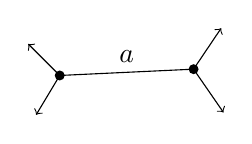
\begin{tikzpicture}[scale=1]
\fill (0,0) circle (1.8pt);\fill (1.7,0.08) circle (1.8pt);
\draw (0,0)--node[above]{$a$}(1.7,0.08);
\draw[->] (0,0)--(-.4,.4);\draw[->] (0,0)--(-.3,-.5);
\draw[->] (1.7,.08)--(2.05,.6);\draw[->] (1.7,.08)--(2.08,-.47);
\end{tikzpicture}}
correspondant à la donnée d'un ens \deleted{$\unsure{E|I}$}\inserted{$I$} de cardinal 4, et d'une partition de type $(2,2)$ de $I$, i.e. à la donnée d'un \uline{carré} combinatoire $\unsure{Q|C}$ (dont $I$ est l'ens des sommets, et la partition est celle des diagonales). \unsure{On notera|On note}
\mspage{12}
